
\documentclass[a4paper, 10pt]{article}
\usepackage {amsmath}
\usepackage{amsfonts}
\usepackage{esint}
%\usepackage{fullpage}
\usepackage{a4wide}
\usepackage[utf8]{inputenc} 
\usepackage[francais]{babel}
\usepackage{fancyhdr}
\usepackage{graphicx}
 \usepackage[all]{xy}

\newtheorem{de}{Définition}[subsection] % les definitions et les theoremes sont
\newtheorem{theo}{Theoreme}[section]    % numerotes par section
\newtheorem{prop}[theo]{Proposition}    % Les propositions ont le meme compteur
                                        % que les theoremes

\DeclareMathOperator{\tr}{tr}

\lhead{} 
\chead{} 
\rhead{\bfseries Méthodes des différences finies} 
\lfoot{JCT }
%\cfoot{} 
%\rfoot{\thepage}

\pagestyle{fancy}

\begin{document}

\section{Distribution de température dans une ailette de radiateur}

Notre but est de déterminer la distribution de température dans une ailette d'un radiateur
de processeur fabriqué en aluminium caractérisé par un conductivité thermique $k_{th}$, une
masse volumique $\rho$ et une capacité calorifique $C$.
La surface du système échange de la chaleur avec l’air ambiante par convection. On note $h$
le coefficient d'échange et $T_a$ la température ambiante.


\begin{figure}[!h]
\centering
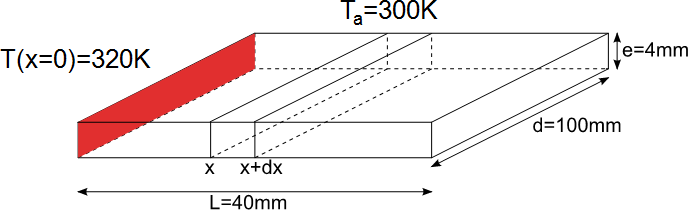
\includegraphics[scale=0.5]{ailette.png}
\caption{ailette}
\label{ailette}
\end{figure}

\begin{table}[!h]
\centering
\begin{tabular}{|l|c|c|}
  \hline
Conductivité thermique & 237 & $W m^{-1} K^{-1}$ \\
Masse volumique & 2700 & $kg  \ m^{-3}$ \\
Capacité calorifique & 897 & $J kg^{-1} K^{-1}$\\
Coefficient de convection & 10 ou 200 & $W m^{-2} K^{-1}$ \\ 
Température ambiante & 300 & $K$ \\ 
  \hline
\end{tabular}
\end{table}

\subsection{Condition d'homogénéité de la température dans l'épaisseur}

Dans la limite des systèmes plats où l'épaisseur est très petite par rapport aux autres dimensions
latérales, la distribution de température est pratiquement homogène dans l'épaisseur. 
Les échanges avec l'air ambiant ne se font principalement qu'à travers les grandes surfaces horizontales.

\begin{figure}[!h]
\centering
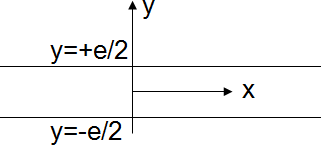
\includegraphics[scale=0.5]{schema2D_ailette.png}
\caption{coupe Oxy de l'ailette}
\label{ailette}
\end{figure}

\begin{enumerate}

\item Montrer en procédant à un D.L. et en appliquant la condition de Neumann que la température le long de l'épaisseur varie selon:

\begin{equation}
T\left( {x,0} \right) = T\left( {x,\;\frac{e}{2}} \right) +\frac{e h}{2 k_{th}}\left( {T\left( {x,\;\frac{e}{2}} \right) - {T_a}} \right) + \vartheta \left( {{e^2}} \right)
\end{equation}

\item En déduire que la distribution tend à devenir homogène selon l'épaisseur si le nombre de Biot
$Bi = \frac{e}{2}\frac{h}{{{k_{th}}}} \ll 1$.

\end{enumerate}

\subsection{Equation de la chaleur transformée}

\begin{enumerate}
\item En faisant un bilan énergétique du flux de chaleur à travers les surfaces d'un petit volume de controle
(voir Fig. \ref{VC}), montrer que l'équation de la chaleur pour des systèmes de faible épaisseur comporte
un terme source supplémentaire.

\begin{figure}[!h]
\centering
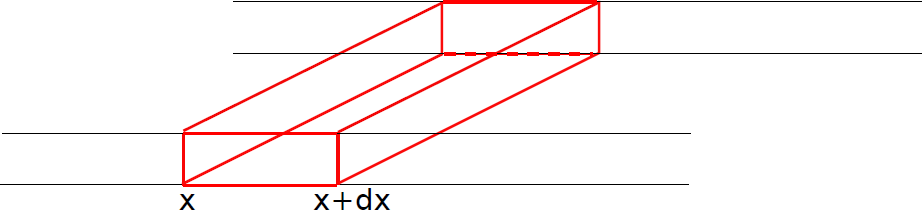
\includegraphics[scale=0.3]{ailetteVcontrol.png}
\caption{volume de controle}
\label{VC}
\end{figure}

\begin{equation} \label{Therm}
- \frac{\partial }{{\partial x}}\left( {{k_{th}}\,\frac{\partial }{{\partial x}}T\left( {x,t} \right)} \right) + \frac{{2h}}{e}\left( {T\left( {x,t} \right) - {T_a}} \right)\, + \rho c\frac{{\partial T}}{{\partial t}}\left( {x,t} \right) = 0
\end{equation}

%\item En général $k_{th}$ dépend de la température, récrire l'équation de la chaleur sachant que
%$$\partial_x k_{th}=\frac{\partial k_{th}}{\partial T}\,  \partial_x T$$
\end{enumerate}

Dans la suite de l'exercice, on négligera la dépendance en température du coefficient de diffusion.

\subsection{Schéma temporelle}

Le système $1D$ repose sur une grille régulière de pas $\Delta x$.  Un indice $p \in [1..N]$ 
repère chaque noeud de la grille d'abscisse $x_p=(p-1) \Delta x$;  Les noeuds extrémités
étant les noeuds $1$ et $N$.  

Le temps est lui-aussi discrétisé en pas $\Delta t$. L'indice $n \ge 0$ repère chaque instant tel que
$t=n \Delta t$. 

La méthode des différences finies revient à remplacer les dérivées temporelles et spatiales par
leur accroissement à partir de développements limités de Taylor.

Deux grandes classes de schémas sont utilisés en différences finies. Ils sont d'ordre $1$ en temps et d'ordre $2$ en espace:
\begin{enumerate}
\item explicite : les dérivées spatiales sont estimées à l'instant $n$. Une suite récurrente en chaque
noeud permet de faire évoluer le temps de l'instant $n$ à l'instant $n+1$. Le schéma est stable
sous condition pour l'équation de la chaleur.  
\item implicite :  les dérivées spatiales sont estimées à l'instant $n+1$. Le passage de l'instant
$n$ à l'instant $n+1$ nécessite la résolution d'un système d'équations linéaires. Le schéma
est inconditionnellement stable pour l'équation de la chaleur.
\end{enumerate}

On vous propose ici d'implémenter un schéma explicite pour l'équation de la chaleur modifiée.
\begin{enumerate}
\item Montrer que pour les noeuds intérieurs tels que $p \in [2..N-1]$, on a :

\begin{equation}\label{sch1}
T_p^{n + 1}  = T_p^{n} -\frac{\Delta t}{\rho \; c} \left( -k_{th} \frac{T_{p+1}^n+T_{p-1}^n
-2 T_{p}^n}{ \left( \Delta x \right)^2 } + \frac{2h}{e}(T_p^n-T_a) \right)
\end{equation}

\item Pourquoi ce schéma n'est pas utilisable pour les noeuds $1$ et $N$? 
\item Comment faut-il le modifier pour traiter aussi bien des conditions de type Dirichlet ou Neumann
homogène $\partial_n T=0$ à gauche comme à droite?

\end{enumerate}

\subsection{Implémentation}

Télécharger le projet source se trouvant sous :\\
\tt{/users/commun/respg/phelma\_2/04\_MDF\_explicite/ailette} \rm \\

\begin{enumerate}
\item Compléter la fonction \tt{explicite.m} \rm

\item Proposer en ensemble de jeux de conditions aux limites permettant de valider votre programme.


\item Montrer que la distribution d'équilibre en appliquant une condition de Dirichlet à gauche et Neumann à droite suit la loi:
\begin{equation}\label{sch1}
T(x)=\left( {{T_{dg}} - {T_a}} \right)\;\frac{{ch\left( {r\left( {x - L} \right)} \right)}}{{ch\left( {r\,L} \right)}} + {T_a}
\end{equation}
avec 
$r = \sqrt {\frac{{2h}}{{e\,{k_{th}}}}} $. Dans quelle limite peut-on la retrouver avec ce schéma numérique?
\end{enumerate}
\end{document}
